\section{Discussion}
\label{sec:chromium-discussion}


% Overall, we see that test flakiness affects Chromium's CI as in other large software systems. It is now well-established thanks to previous research studies~\cite{Luo2014,Lam2019RootCausing} and industrial reports~\cite{Micco2017,FlakinessSpotify} that flaky failures force developers to spend time on false alerts which are difficult to reproduce and debug. As they lose trust in their test suite results, they stop relying on test signals and end up integrating buggy features in the main codebase. 
% In an attempt to mitigate the problem, important attention has been given by the research community towards flaky test detection, with the goal of helping developers find flaky tests more efficiently than with the rerunning approach. \\
% \revise{\textbf{\textit{On the importance to practitioners:}}} In our case study, we make an important finding: flaky tests are not always giving false signals, as a substantial \nicefrac{1}{3} of regressions are reported by tests that happened to flake in other builds. 
% This is even more problematic when considering the fact that \nicefrac{3}{4} of failing builds only list flaky tests as fault-revealing tests. This means that signals from flaky tests should be considered and treated carefully. 
% We also noted a very low precision of our model in RQ1. This means that there are many false positives (\ie non flaky tests mislabelled as flaky tests). This is a worrying aspect in the two scenarios such a model can be used in the CI: (1) if the classifier is used to discard information coming from flaky tests, it would convince developers to not consider important signals (\eg a fault-revealing test). (2) If the model is used to find flaky tests to help developers debug them, this would require them to investigate many tests that are actually not flaky. 
% Our findings diminish the purpose of flaky test detection in the context of continuous integration: that is when detection tools are used to predict if tests are flaky or not. On the contrary, it advocates the use of tools towards the detection of failures when they occur and being able to classify them as flaky or legitimate.

% \subsection{Prevalence of regressions identified by flaky tests} 
We seek to better understand the results showing that existing approaches targeting the detection of flaky tests missed a non-negligible part (76.2\%) of fault-triggering failures by classifying them as flaky. To do so, we investigate the following aspects regarding \textit{the entire dataset}.

We first report general information about the prevalence of flaky tests and fault-revealing tests in order to have a better view of the failures occurring in each build. Then, we report the number of fault-revealing tests also found as flaky by the Chromium CI (reruns) in other builds (we further refer to them as fault-revealing flaky tests). Finally, we also check for the number of failing builds that only contain fault-revealing flaky tests. We consider these builds important since the related faults are not detected by any non-flaky test and would be missed if flaky test detectors were used.

% Figure Tests per Build
\begin{figure}[!htbp]
\centering
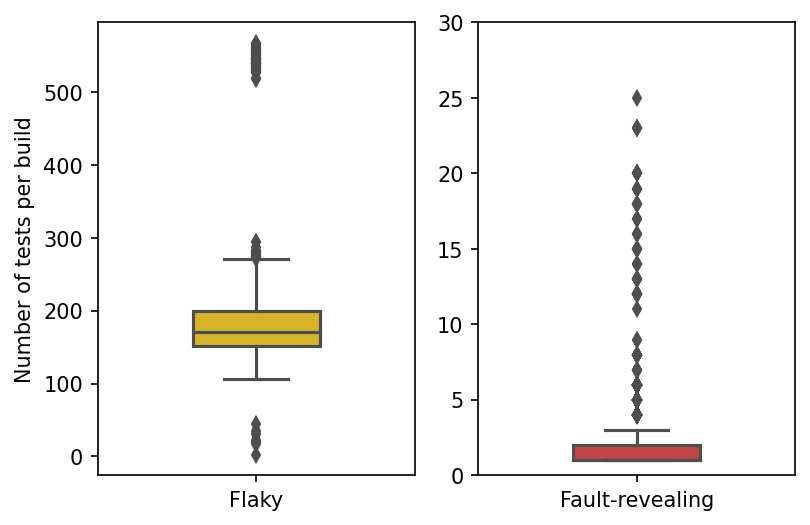
\includegraphics[width=0.8\textwidth]{figures/chromium/testsPerBuild.png}
\caption{Number of flaky tests and fault-revealing tests per build. On average, there are 250 flaky tests per build and 1 fault-revealing test per failing build.}
\label{fig:testsPerBuild}
\end{figure}

Figure~\ref{fig:testsPerBuild} shows the distribution of flaky tests and fault-revealing tests in the studied builds. We observe that there is an average of 178 flaky tests per build with a low standard deviation (41), showing that flakiness is prevalent in the Chromium CI. In the case of fault-revealing tests, taking into account all builds would result in an average number of tests close to 0 as a majority of builds are exempt from them. Thus, for better visualisation, we only considered builds containing at least one fault-revealing test (\ie failing builds). The average number of fault-revealing tests per failing build is 2.7.
%, which is why we dot see the lower quartile in the Figure. 
The standard deviation for fault-revealing tests is 14.9 and the number of fault-revealing tests reported in one build goes up to 579 in our dataset.

\begin{table}[ht]
\caption{Number of builds containing each studied test type. All builds contain flaky tests. \nicefrac{1}{4} contain fault-revealing tests. Among the failing builds, \nicefrac{3}{4} contain only fault-revealing tests that are flaky in other builds.}
\label{table:DiscBuilds}
\centering
\begin{tabular}{c|c} 
 \toprule
 \textbf{Builds containing} & \textbf{Number} \\ [0.5ex] 
 \midrule
 Flaky tests & 10,000 \\ 
 Fault-revealing tests & 2,415 \\ 
 Fault-revealing flaky tests & 1,974 \\ 
 Exclusively fault-revealing flaky tests & 1,766 \\ 
 \bottomrule
\end{tabular}
\vspace{-1em}
\end{table}

Table~\ref{table:DiscBuilds} provides, for each type of test, the number of builds that contain at least one instance of this type. We note that all builds contain at least one flaky test (a test that flaked during this build). In Chromium CI, flaky tests are non-blocking and will not cause a build failure. That is, tests flaking within the build are ignored during this build. 

Developers are expected to investigate test failures only when they occur consistently across 5 reruns (resulting in a fault-revealing test). Such fault-revealing tests occur in 24.15\% of the builds (i.e. in 2,415 builds). Interestingly, 1,974 of these builds (i.e. 81.73\%) contain fault-revealing tests that flaked in previous builds, indicating that \emph{tests with a flake history should not be ignored in future builds}. Perhaps worse, in 1,766 builds \emph{all} fault-revealing tests have flaked in some previous builds, indicating that no "reliable" tests identified the fault(s).

% \begin{table}[ht]
% \caption{Information about tests. 22,477 tests are exclusively flaky among all builds. 2,343 tests are fault-revealing, among which \nicefrac{1}{3} are flaky in other builds.}
% \label{table:rq1tests}
% \begin{center}
% \begin{tabular}{|c|c|c|} 
%  \hline
%   & \textbf{Number} & \textbf{Ratio} \\ [0.5ex] 
%  \hline
%  Tests & 209,530 & 100\% \\ 
%  Passing tests & 198,273 & 94.6\% \\ 
%  Exclusively passing tests & 184,710 & 88.2\% \\ 
%  Flaky or Fault-revealing tests & 24,820 & 11.8\% \\ 
%  Exclusively flaky tests & 22,477 & 10.7\% \\ 
%  Exclusively fault-revealing tests & 1,446 & 0.7\% \\ 
%  Fault-revealing flaky tests & 897 & 0.4\% \\ 
%  \hline
% \end{tabular}
% \end{center}
% \end{table}

% Figure Venn diagram
\begin{figure}[!htbp]
\centering
%\vspace{-0.5m}
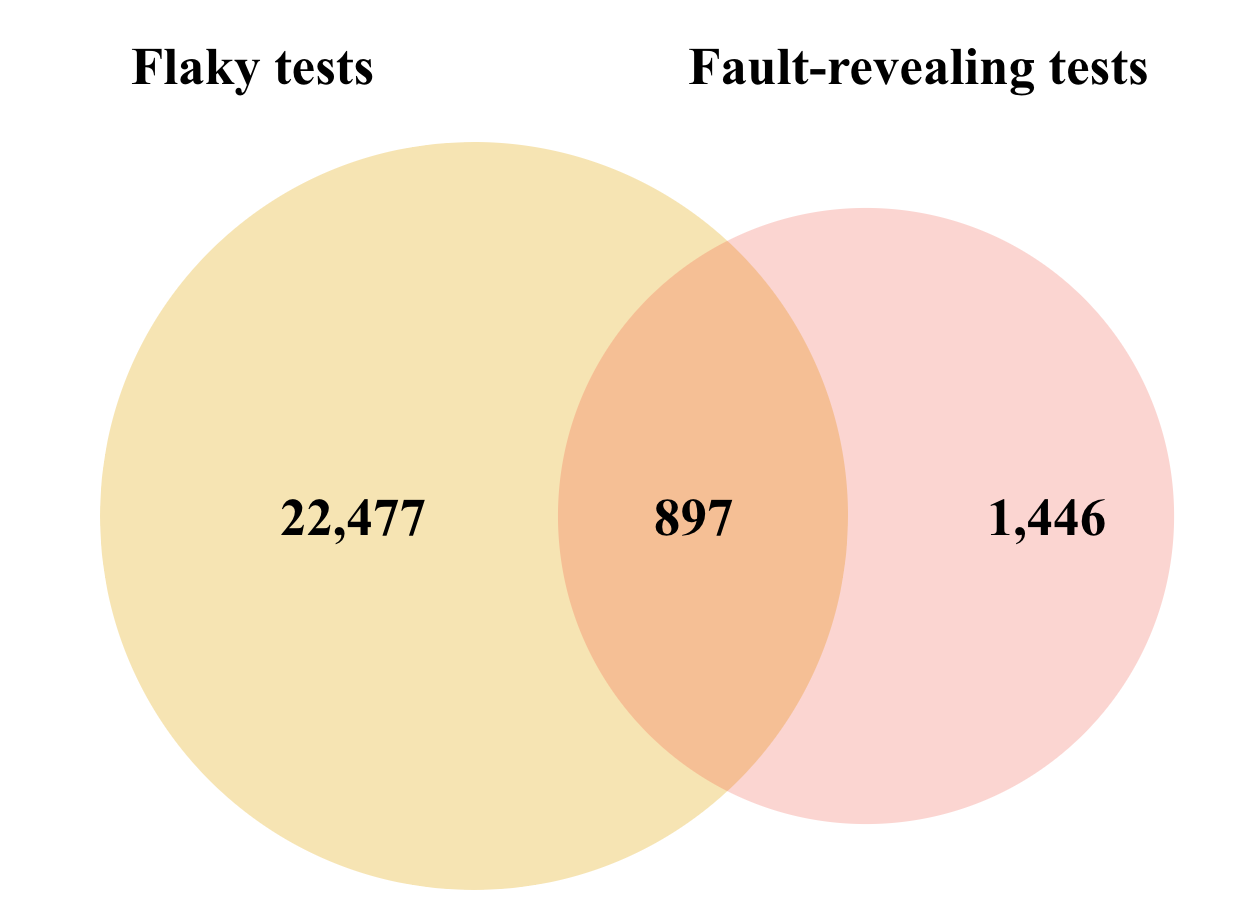
\includegraphics[width=0.8\textwidth]{figures/chromium/venn.png}
\vspace{-1em}
\caption{Distribution of tests in our dataset. 22,477 tests are exclusively flaky among all builds. 2,343 tests are fault-revealing, among which \nicefrac{1}{3} are flaky in other builds.}
\label{fig:venn}
\vspace{-0.7em}
\end{figure}

By investigating the status of all tests across all builds -- see Figure~\ref{fig:venn}. Among the 209,530 tests of the Chromium project, 24,820 have failed in at least one build, including 22,477 that were always flaky. Thus, 2,343 tests were fault-revealing in at least one build, i.e., they attested the presence of faults, 897 were also flaky in at least one other build. That is, \emph{38.3\% of tests that have been useful to detect faults have also a history of flakiness}.

%'We visually represent the set of flaky tests and fault-revealing tests using the Venn diagram in Figure~\ref{fig:venn}. Across the 10,000 builds in our dataset, we find 2,343 fault-revealing tests. Among them, 1,446 are exclusively fault-revealing, \ie they were never found to be flaky in other builds. On the contrary, 897 fault-revealing tests were marked as flaky in at least one other build. This represents \nicefrac{1}{3} of fault-revealing tests.
%% that most of the 209,530 tests in our dataset are passing tests with 88.2\% having not failed once over the 10,000 builds we collected. Regarding failures, 24,820 tests were found to be flaky or failing in one or more builds. Among them, a majority, \ie 90\%, are exclusively flaky.  Interestingly, 2,343 tests are fault-revealing tests, \ie 1.1\%. Among them, \nicefrac{1}{3} exhibit both flaky and failing behaviour as they were reported as flaky in one or more other builds. \\

\begin{tcolorbox}[
    left=2pt,right=2pt,top=2pt,bottom=2pt, %margin  
    arc=0pt, % corners
    boxrule=1.2pt % line width
]
Flakiness affects all Chromium CI builds and mixes critical (fault-revealing) signals with false (flakiness) signals. Indeed, 81.7\% of builds contain fault-revealing tests that were flaky in some previous builds, and 38.3\% of all tests flake in some builds and reveal faults in other builds. 
%\textbf{RQ1:} In the Chromium CI, flaky tests are frequent in all builds. Critically, an important \nicefrac{1}{3} of regressions are reported by fault-revealing flaky tests. In addition, almost \nicefrac{3}{4} of failing builds exclusively contain regressions found by flaky tests (fault-revealing flaky tests). 
\end{tcolorbox}